Now that the requirements are set, and our research question has been formulated, we know what type of features we are looking for in a technical setting. In this section we illustrate our findings, and justify our choices in terms of tools deployment, architecture design and system components.

\subsection{Why a web application?}
One of the main ideas that have been advised to us by our coach is the creation of a web application for our project. The justification for this is ease of usability and compatibility across several platforms. Web applications are also exempted from platform-specific updates, whereas now one single update on the web application immediatly reaches all of our users at once. When a web application is used, users can access the exact same content from different computers or mobile devices.

\subsection{Objective}
There are various frameworks available for the implementation of a web application. The choice of a specific framework usually depends on the context and objectives of the project itself. Our current project entails the development of a prototype within a time constraint of 11 to 12 weeks, which persuaded us to use a full stack framework. If we would use a full stack framework, we should be able to focus primarily on techniques that allow us to perform rapid prototyping, generate quality code and provide good documentation all of which meet the clients requirements. The following features should facilitate reaching our objectives during the development phase.

\begin{enumerate}
	\item \textbf{a Full-Stack framework}: A framework that already contains all the basic utilities to create and run an application, with the option to connect or import external entities too.
	\item \textbf{Rapid Prototyping}: Allows us to convert the clients requirements into a prototype in a fast way so it can be immediatly reviewed and refined for the next prototype.
	\item \textbf{Scalability}: The ability of a system, network, or process to handle a growing amount of work in a capable manner or its ability to be enlarged to accommodate that growth.\cite{wiki:scalability}
	\item \textbf{Reliablity}: The ability of a system to function under predefined conditions.
\end{enumerate}
\subsection{Project Development Methodology} % (fold)

For our project development methodology we chose the agile Scrum methodology. This means that we will have weekly sprints (iterations within a fixed amount of time) in which a predefined set of items, taken from a product backlog\footnote{The agile product backlog in Scrum is a prioritized features list, containing short descriptions of all functionality desired in the product.\cite{backlog} }, are to be implemented. Each week we show our client what we achieved, and we discuss possible changes (within the requirements that have been agreed upon). The Scrum method gives developers an advantage over sequential methodologies such as the waterfall model or the V-model, because when changes have to be made to either pieces of code, features or even requirements, the sequential methodologies force the developers to revise (or even redo) everything that happened after the point where they were processed within the implementation. These sort of changes are more manageable within iterative methodologies such as Scrum. Scrum also allows developers to uncover designing constraints that may not have been obvious at the start of the implementation by giving them the opportunity to pivot after every sprint. \\\\
Given these advantages, the use of the Scrum method should be the most adequate for our project. When using Scrum, some roles and conventions have to be attributed, which are listed below:

\begin{enumerate}
	\item \textbf{Roles}
		\begin{itemize}
			\item Product Owner/Dev Team: Arnaud Hambenne
			\item Scrum master/Dev Team: Soheil Jahanshahi
			\item Client: TU Delft Library (Babak Dehghenpour, Nicoleta Nastase)
			\item Coach: Alberto Bacchelli
		\end{itemize}
	\item \textbf{Conventions}	
\begin{itemize}
		\item Sprint duration: One week.
		\item Sprint Planning meeting: A weekly meeting that is used to prioritise the selected features for each sprint. 
		\item Sprint reflection report: A weekly evaluation where the estimated effort is compared to the actual effort that was needed to implement the chosen features, and where possible issues are documented. The evaluation takes place at the end of each Sprint.
		\item Daily Scrum meeting: A daily meeting between the developers which takes about 15 minutes.
		\item Sprint review meeting: A weekly meeting of about 15-20 minutes with the clients, in order to receive their feedback on the implemented features.
\end{itemize}
\end{enumerate}

\subsubsection{Definition of Done} 
For this project, we have defined an extra convention for ourselves



For this project, we define a convention called the definition of done, A project task is done if the following holds for the task:

\begin{itemize}
	\item	Implemented (the code has been written)
	\item	Unit tested (JUnit test cases)
	\item 	Integrated
	\item 	Integration tested
	\item 	Documented (the change has been documented)
\end{itemize} 

\subsection{Architectural Model : MVC}
Having a design pattern is important when you want to write re-usable and maintainable code.
For the `Virtual Assistant' application we decided that it is best to divide the application into three interconnected parts which separate the internal representation of data from information that is presented to the users\cite{wiki:mvc}. This type of designpattern is called the MVC pattern. MVC stands for the three components that make up the pattern, the Model, the View and the Controller.
\begin{figure}[h]
\centering
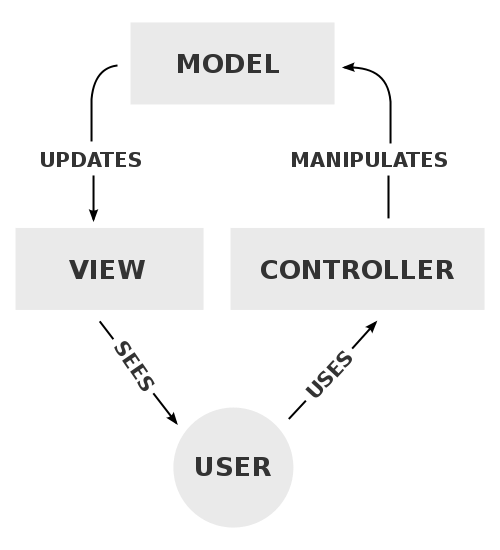
\includegraphics[scale=0.3]{./img/MVC.png}
\caption{\small{The Model, View and Controller, interconnected by directed edges}}
\label{mvc}
	
\end{figure}

As shown in fig \ref{mvc}, the MVC separates the application into a front end, the View, and a back end, the Model and Controller. The Controller provides the link between both the View and the Model, which makes it act as the brain of the application. The Controller decides what the user input was and how the Model needs to change as a result of this input\cite{codinghorror}. The Controller then responds back to the user by calling the resulting View.

\subsection{Choice of framework}
In order to be able to choose a suitable web application framework, we have defined some  constraints for ourselves that we can use to benchmark various popular existing frameworks. Our first criteria was choosing a framework which is based on either Java, Scala or Javascript. With this in mind, we have narrowed our choices down to four popular frameworks such as \href{https://grails.org/}{Grails}, \href{https://vaadin.com/home}{Vaadin}, \href{https://www.playframework.com/}{Play!} and \href{http://projects.spring.io/spring-framework/}{Spring}. Finally we were able to boil down our choice to either the Spring framework or the Play! framework.
\subsubsection{Benchmarking}
 The table below lists the comparison of these two frameworks within the constraints that we have defined:\\\\

\begin{center}
	

\begin{tabular}{ |l||l| C{6cm} | C{6cm} |  }
 \hline
 \multicolumn{4}{|c|}{\textbf{Benchmark Table}} \\
 \hline
 ~ & \textbf{Constraint} & \textbf{Play! Framework} & \textbf{Spring Framework}\\
 \hline
 1 & Development Principles & Convention over configuration, Don't repeat yourself, Test-driven development & Convention over configuration, Don't repeat yourself, Test-driven development, Domain Driven Design \\
 \hline
 2 & Design pattern & Model-View-Controller, Dependency-injection, Active-Record, DAO, Actors & Model-View-Controller, Dependency-injection, Domain-Driven-Design \\
 \hline
 3 & Operating System & Cross-Platform & Cross-Platform \\
 \hline
 4 & Programming Language & Java, Scala & Java \\
 \hline
 5 & Database & MySQL, PostgreSQL, MongoDB, Oracle, SQLite, HBase, H2-database, Resis & Microsoft-BI, MYSQL, PostgreSQL, Oracle, SQLite, IBM-DB2, JDBC-Compatible, MongoDB, Microsoft-SQL-Server, Taradata, Cassandra \\
 \hline
 6 & Database model & NoSQL, Relational, Object-Relational & Document-Oriented, Graph-Oriented, Multidimensional, NoSQL, Relational, Object-Relational, XML Database \\
 \hline
 7 & Documentation level & Excellent&Excellent \\
 \hline
 8 & Programming paradigm & OOP, Functional, Concurrency Oriented&Aspect-Oriented, OOP \\
 \hline
 9 & Cloud Platform Support & Heroku, Clever Cloud, Amazon EC2, Cloud Bee, OpenShift, digital Ocean, playframework Cloud & Open Shift, Heroku, Amazon EC2, AppHarbor, CloudBee \\
 \hline
 10 & Annotation support & YES & YES \\
 \hline
 11 & Scalability & YES & YES \\
 \hline
\end{tabular}
\end{center}

The result of this benchmark shows us that the differences between these two frameworks are fairly minimal. We decided to use the Play!Framework for this project.
\newpage

\subsection{Play! Framework}
  One of the main reasons we selected the Play! Framework is because this framework has been proven in production. For example the LinkedIn web application has been developed using the Play! Framework. The following figure\ref{play} illustrates an overview of the Play! Framework.\\
\begin{figure}[h!]
\centering
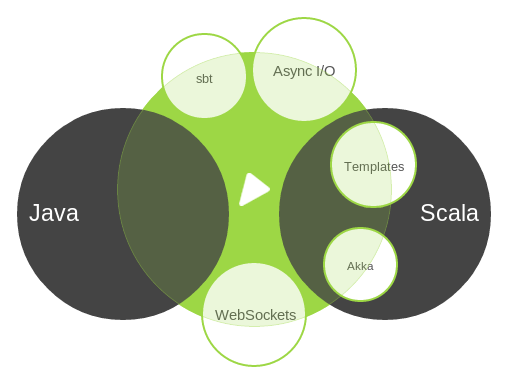
\includegraphics[scale=0.5]{./img/play.png}
\caption{\small{The main attributes and features of the Play! Framework}}
\label{play}
\end{figure}
 
 
The Play! Framework offers excellent documentation\cite{playDoc} that can help us get familiar with the Play! environment. First of all, it is an open source application that has an amazing error handling because of the fact that everything is compiled and built on the fly. This makes it easier for developers to detect bugs and can dramatically improve the developer's productivity to make changes. By reloading the browser, you can immediately see the changes you just made, which makes it perfect for fast prototyping within our project. Moreover, Play! supports both the Scala and Java languages, it comes with a Scala template that allows you to write dynamic code within an HTML body, and it also comes with pre-configured testing support. This last one is particularly important because that means we do not need to worry about adding Junit dependencies to the build file. \\\\
Play! also offers the use of the EBean server interface which is very handy for fetching and saving beans to a particular DataSource. It can make reactive applications simpler because Play! is built on \href{http://netty.io/}{Netty}, which means it supports non-blocking I/O.\footnote{ non-blocking I/O is a form of input/output processing that permits other processing to continue before the transmission has finished.} This will enable our web application to make remote calls inexpensively which is crucial for high performance web applications.

\newpage








% \begin{enumerate}
% 	\item User(Client) interaction with web(Asynchronous vs sync)
% 	\item Distributed application structure(client/server)
% 	\item Scalability is the ability of a system, network, or process to handle a growing amount of work in a capable manner or its ability to be enlarged to accommodate that growth.
% 	\item Build systems
% 	\item Databases(need more research)
% 	\item Continuous Integration
% \end{enumerate}
% \subsubsection{Synchronous Vs Asynchronous}
% \subsubsection{Server-Side Rendering Vs Client/Server}
% \subsubsection{Vertical Scalability Vs. Horizontal Scalability}
% \subsubsection{sbt Vs. Maven}
% \subsubsection{mongodb vs nosql vs mysql vs postgres}
% \subsubsection{Template}
% \subsubsection{Testing}
% \subsubsection{Jenkins}
% \subsubsection{frameworks}

